\labwork{Установка ПО ST-Link для \vld}\label{labinststsoft}

\menu{\wcmd{\url{http://www.google.com}}>ST-Link>ST-Link - STMicroelectronics}

\bigskip
\begin{tabular}{l l l}
\menu{STSW-LINK002>Download}	&ST-LINK USB driver for Windows XP&драйвер\\
\menu{STSW-LINK004>Download}	&STM32 ST-LINK utility&ПО программатора\\
\end{tabular}

\bigskip
\menu{\file{st-link\_usbdriver.zip}>\file{ST-Link\_USBdriver.exe}}

\menu{STLinkDriver>Welcome>Next>Install
to>\file{C:/ARM/STM32/STdriver}>Next>Install>Finish}

\bigskip
\menu{\file{stsw-link004.zip}>\file{STM32 ST-LINK Utility\_v3.4.0.exe}}

\menu{ST-LINK
Utility>Next>License>Yes>Distination>\file{C:/ARM/STM32/STLinkUtil}>Finish}

\menu{(сам запустился) Device Driver Install Wizard>Далее>Установить}

\bigskip
\menu{\winstart>STMicroelectronics>ST-LINK Utility>STM32 ST-Link}

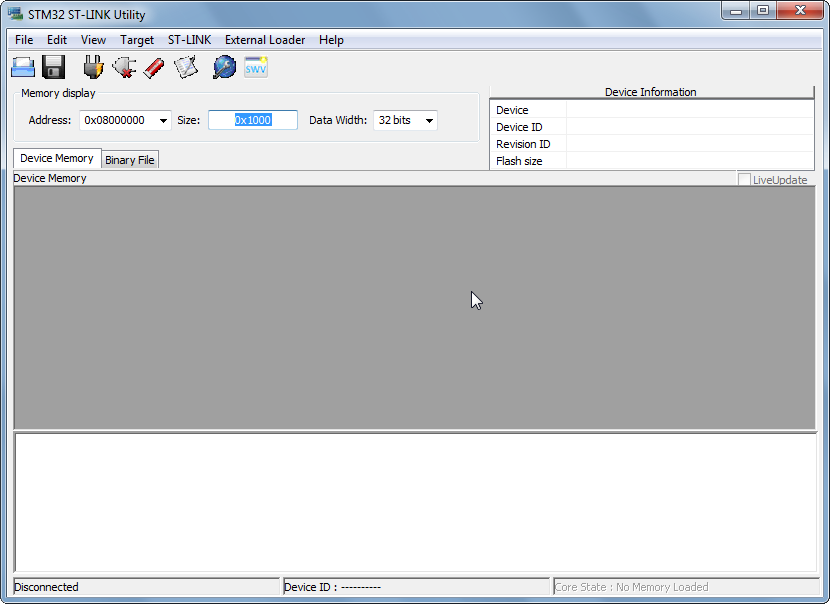
\includegraphics[height=0.5\textheight]{fig/stlink0.png}

\bigskip
\menu{STutil>Target>Connect}

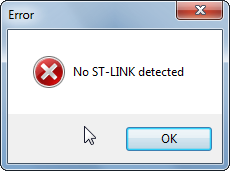
\includegraphics[height=0.2\textheight]{fig/nostlink.png}

\bigskip
Подключаем плату \vld\ кабелем, в системе подключается новое устройство,
на плате запускается ранее залитая в МК прошивка:

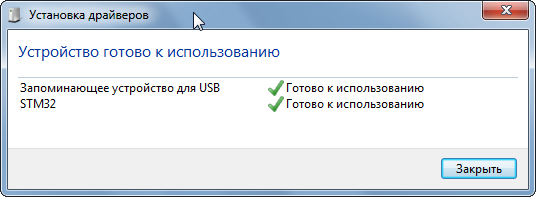
\includegraphics[height=0.3\textheight]{fig/stdrvok.png}

\bigskip
\menu{STutil>Target>Connect}

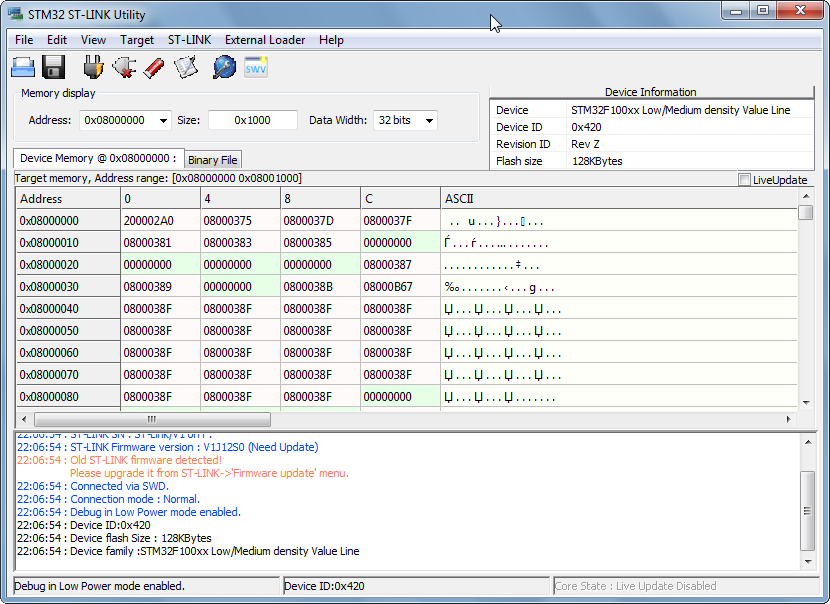
\includegraphics[width=0.9\textwidth]{fig/stconnected.png}

\bigskip
Обновление прошивки ST-Link:

\menu{ST Link>ST-LINK>Firmware update>Device Connect>not in DFU
mode}

\menu{передергиваем плату>Device connect>Upgrade to V.1.J13.S0>Yes}

\bigskip
Установка GDB-сервера для STLink:
\cp{\url{http://www.emb4fun.de/archive/stlink/index.html}}

\bigskip
Для отладки программ для МК STM32F нужно установить
пакет с \url{https://github.com/texane/stlink}.  
Поскольку на гитхабе лежат исходники, качаем бинарную сборку под win32
c \url{http://www.emb4fun.de}:

\bigskip
\menu{\wcmd{\url{http://www.emb4fun.de/archive/stlink/download/stlink-20130324-win.zip}}}

\menu{file{stlink-20130324-win.zip}>\file{D:/ARM/STM32/stlink-20130324-win}}

Прописать пусть в \verb|$PATH|

\alarm{Подключить \vld}

Для работы нужен спецдрайвер совместимый с libusb, поэтому

\menu{\url{http://zadig.akeo.ie/}>\url{http://zadig.akeo.ie/downloads/zadig\_2.1.0.exe}}

\menu{\file{zadig\_2.1.0.exe}>Zadig update>No}

\menu{Options>List all devices>STM32 STLink>USB ID 0483:3744>Replace driver}

\menu{Warning System Driver>Yes>Driver was installed>Close}

Запускаем \menu{\wcmd{cmd}}

\begin{lstlisting}[style=con]
C:\Users\dmitry>st-util -1 -m -p 1234
STLINK GDB Server v0.5.6 (Mar 24 2013 10:29:19)
Many thanks to the STLINK development team.
(https://github.com/texane/stlink)

2014-07-20T18:55:59 INFO src/stlink-common.c: Loading device parameters....
2014-07-20T18:55:59 INFO src/stlink-common.c: Device connected is: F1 Medium-den
sity Value Line device, id 0x10016420
2014-07-20T18:55:59 INFO src/stlink-common.c: SRAM size: 0x2000 bytes (8 KiB), F
lash: 0x20000 bytes (128 KiB) in pages of 1024 bytes
2014-07-20T18:55:59 INFO src/stlink-sg.c: Successfully opened a stlink v1 debugg
er
Chip ID is 00000420, Core ID is  1ba01477.
KARL - should read back as 0x03, not 60 02 00 00
Listening at *:1234...
\end{lstlisting}

\bigskip
\menu{Run>Run configurations>C/C++ Application>\rms>New}

\menu{Name:>ST-Link}

\menu{Main>C/C++
Application:>\file{C:/ARM/STM32/stlink-20130324-win/bin/st-util.exe}>Disable
auto build}

\menu{Arguments>-1 -p 1234 }

\menu{Common>Display in>\checkbox\ Run} 

\menu{Apply>Close}


